\setcounter{chapter}{19} % Chapter 19
\chapter{Miscellaneous Topics and Motivation}

\section{Geometric Motivation: Why Abstraction Matters}

It is a common temptation to simply identify every $n$-dimensional vector space over $K$ with the standard coordinate space $K^n$. However, while they are algebraically isomorphic for any fixed parameter, they may not be "continuously" isomorphic when the vector spaces depend dynamically on parameters.

\subsection{The Möbius Vector Bundle}

\begin{definition}[A Continuous Family of Subspaces]
  Let $S \subseteq \mathbb{C}$ be the unit circle defined by $S = \{e^{i\theta} \mid \theta \in [0, 2\pi]\}$. For each $z = e^{i\theta} \in S$, we define a 1-dimensional subspace $L_z \subseteq \mathbb{R}^2$ as follows:
  \[ L_z := \operatorname{Sp} \left( \cos\frac{\theta}{2}, \sin\frac{\theta}{2} \right). \]
\end{definition}

Notice a topological anomaly: $z=1$ corresponds to both $\theta=0$ and $\theta=2\pi$.
In the first case ($\theta=0$), the spanning vector is $(1,0)$, so $L_1 = \operatorname{Sp}(1,0)$.
In the second case ($\theta=2\pi$), the spanning vector is $(-1,0)$, which gives the exact same subspace $L_1 = \operatorname{Sp}(-1,0)$. The line $L_z$ rotates at exactly half the speed of the point $z$.

\begin{center}
  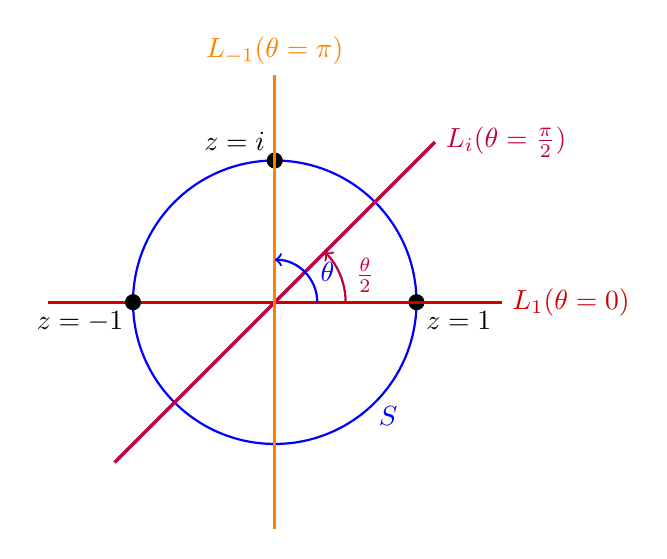
\begin{tikzpicture}[scale=1.8]
    % Background axes
    \draw[gray!40, thin] (-1.5,0) -- (1.5,0);
    \draw[gray!40, thin] (0,-1.5) -- (0,1.5);

    % Unit circle S
    \draw[thick, blue] (0,0) circle (1);
    \node[blue] at (0.8, -0.8) {$S$};

    % theta = 0
    \filldraw[black] (1,0) circle (1.5pt) node[below right] {$z=1$};
    \draw[very thick, red!80!black] (-1.6,0) -- (1.6,0) node[right] {$L_1 (\theta=0)$};

    % theta = pi/2
    \filldraw[black] (0,1) circle (1.5pt) node[above left] {$z=i$};
    \draw[very thick, purple] (-1.13,-1.13) -- (1.13,1.13) node[right] {$L_i (\theta=\frac{\pi}{2})$};

    % theta = pi
    \filldraw[black] (-1,0) circle (1.5pt) node[below left] {$z=-1$};
    \draw[very thick, orange] (0,-1.6) -- (0,1.6) node[above] {$L_{-1} (\theta=\pi)$};

    % Arcs showing the half-speed rotation
    \draw[->, blue, thick] (0.3,0) arc (0:90:0.3) node[midway, right=2pt] {$\theta$};
    \draw[->, purple, thick] (0.5,0) arc (0:45:0.5) node[midway, right=2pt] {$\frac{\theta}{2}$};
  \end{tikzpicture}
\end{center}

\begin{proposition}[Non-triviality of the Möbius Bundle]
  There does not exist a family of linear isomorphisms $T_z \colon L_z \to \mathbb{R}$ that depends continuously on the parameter $z \in S$.
\end{proposition}

\begin{proof}[Proof Sketch]
  Consider the disjoint union of all these lines parameterized by $z$, which forms a space $M = \{ (z, v) \mid z \in S, v \in L_z \}$. Topologically, this forms a vector bundle over $S^1$ known as the Möbius strip.

  If such a continuous family of isomorphisms $T_z$ existed, it would allow us to construct a global homeomorphism $\Phi \colon M \to S \times \mathbb{R}$. Removing the zero-section (the center circle where $v=0$) from both spaces would imply that $M \setminus \{0\} \cong S \times (\mathbb{R} \setminus \{0\})$.

  However, $S \times (\mathbb{R} \setminus \{0\})$ consists of two disconnected cylinders (an "upper" and "lower" half). In contrast, if you cut a Möbius strip down its center line, it remains a single connected piece. This topological contradiction demonstrates that we cannot consistently and continuously identify all $L_z$ with $\mathbb{R}$. Abstraction is therefore necessary to handle "twisted" families of spaces.
\end{proof}

\section{Affine Geometry}

In our strict definition of a vector space, there is always a distinguished origin $0$. Affine geometry studies spaces that "look like" vector spaces locally, but have forgotten their origin.

\begin{definition}[Affine Space]
  A subset $X \subseteq V$ is called an \qt{affine space} if there exists a linear subspace $U \subseteq V$ and a translation vector $x_0 \in V$ such that $X = x_0 + U$.

  We say that $X$ is modeled on the subspace $U$, and we write the \qt{direction space} as $\vec{X} := U$. The elements of $X$ are called \qt{points}, while the elements of $\vec{X}$ are called \qt{vectors}.
\end{definition}

\begin{proposition}[Algebra of Affine Spaces]
  Let $X$ be an affine space modeled on $\vec{X}$. Then:
  \begin{enumerate}
    \item We cannot inherently add two points $p, q \in X$, as $p+q \notin X$ in general.
    \item We can translate a point $p \in X$ by a vector $v \in \vec{X}$ to obtain a new point $p+v \in X$.
    \item For any two points $p, q \in X$, their difference defines a unique vector $\vec{pq} := q - p \in \vec{X}$.
  \end{enumerate}
\end{proposition}

\begin{center}
  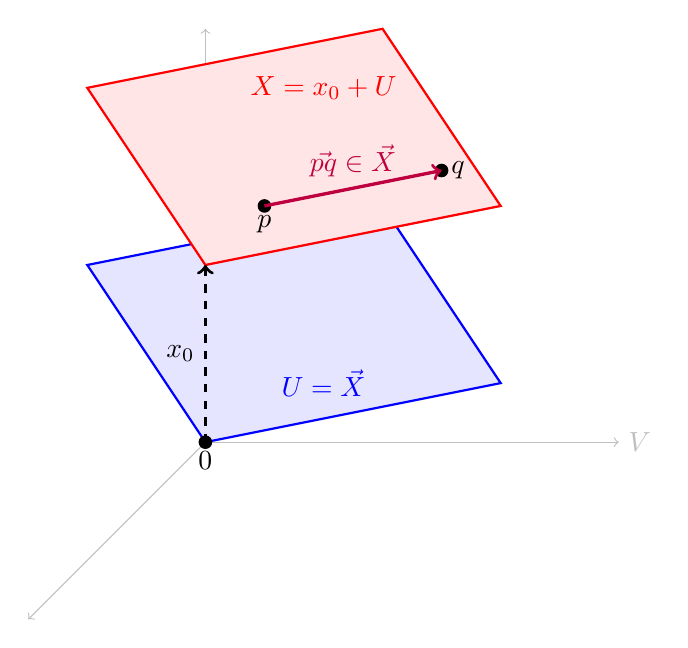
\begin{tikzpicture}[scale=1.5]
    % Axes to imply ambient space V
    \draw[->, gray!50] (0,0) -- (3.5,0) node[right] {$V$};
    \draw[->, gray!50] (0,0) -- (0,3.5);
    \draw[->, gray!50] (0,0) -- (-1.5,-1.5);

    % Subspace U (passing through origin)
    \filldraw[blue!10, draw=blue, thick] (0,0) -- (2.5,0.5) -- (1.5,2) -- (-1,1.5) -- cycle;
    \node[blue] at (1,0.5) {$U = \vec{X}$};

    % Affine space X (displaced)
    \filldraw[red!10, draw=red, thick] (0,1.5) -- (2.5,2.0) -- (1.5,3.5) -- (-1,3.0) -- cycle;
    \node[red] at (1,3) {$X = x_0 + U$};

    % Origin and translation
    \filldraw[black] (0,0) circle (1.5pt) node[below] {$0$};
    \draw[->, very thick, dashed] (0,0) -- (0,1.5) node[midway, left] {$x_0$};

    % Points in X
    \filldraw[black] (0.5, 2.0) circle (1.5pt) node[below] {$p$};
    \filldraw[black] (2.0, 2.3) circle (1.5pt) node[right] {$q$};
    \draw[->, very thick, purple] (0.5, 2.0) -- (2.0, 2.3) node[midway, above] {$\vec{pq} \in \vec{X}$};
  \end{tikzpicture}
\end{center}

\begin{theorem}[Thales' Theorem in Affine Geometry]
  Let $H, H', H''$ be three distinct parallel affine planes in an ambient space $V$. Let $l_1, l_2$ be two affine lines intersecting these planes at the points $p_1, p_1', p_1''$ and $p_2, p_2', p_2''$ respectively. Then:
  \[ \frac{\vec{p_1 p_1''}}{\vec{p_1 p_1'}} = \frac{\vec{p_2 p_2''}}{\vec{p_2 p_2'}}. \]
  Crucially, the ratio of these vectors does not depend on the specific transversals chosen, but only on the relative distances between the parallel planes.
\end{theorem}

\begin{center}
  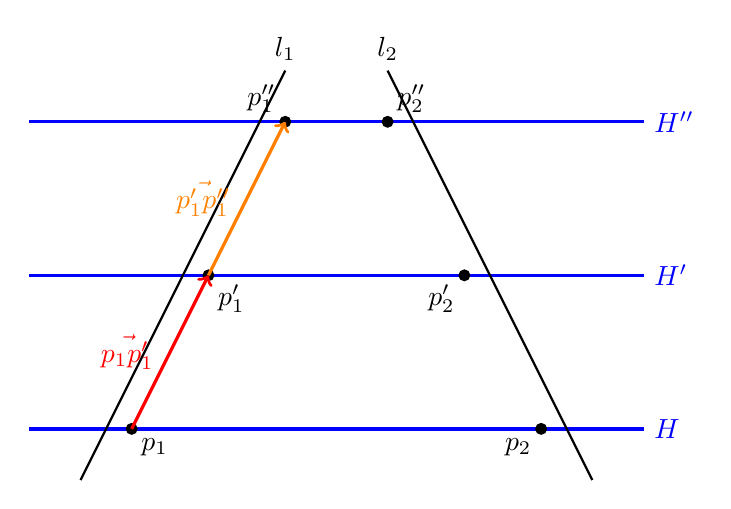
\begin{tikzpicture}[scale=1.3]
    % Parallel planes (represented as lines in 2D projection)
    \draw[very thick, blue] (-1, 3) -- (5, 3) node[right] {$H''$};
    \draw[very thick, blue] (-1, 1.5) -- (5, 1.5) node[right] {$H'$};
    \draw[very thick, blue] (-1, 0) -- (5, 0) node[right] {$H$};

    % Transversal line 1
    \draw[thick, black] (-0.5,-0.5) -- (1.5, 3.5) node[above] {$l_1$};
    \filldraw (0, 0) circle (1.5pt) node[below right] {$p_1$};
    \filldraw (0.75, 1.5) circle (1.5pt) node[below right] {$p_1'$};
    \filldraw (1.5, 3) circle (1.5pt) node[above left] {$p_1''$};

    % Transversal line 2
    \draw[thick, black] (4.5,-0.5) -- (2.5, 3.5) node[above] {$l_2$};
    \filldraw (4, 0) circle (1.5pt) node[below left] {$p_2$};
    \filldraw (3.25, 1.5) circle (1.5pt) node[below left] {$p_2'$};
    \filldraw (2.5, 3) circle (1.5pt) node[above right] {$p_2''$};

    % Vector highlights (corrected)
    \draw[->, very thick, red] (0,0) -- (0.75, 1.5) node[midway, left=2pt] {$\vec{p_1 p_1'}$}; % Vector p1 p1'
    \draw[->, very thick, orange] (0.75, 1.5) -- (1.5, 3) node[midway, left=2pt] {$\vec{p_1' p_1''}$}; % Vector p1' p1''
  \end{tikzpicture}
\end{center}

\section{Introduction to Eigenvalues: Fibonacci Sequences}

\subsection{The Vector Space of Fibonacci Sequences}

Consider the set $Fib \subseteq \mathbb{R}^\infty$ of all infinite real sequences $(a_0, a_1, a_2, \dots)$ that satisfy the linear recurrence relation $a_n = a_{n-1} + a_{n-2}$ for all $n \ge 2$.

\begin{proposition}[Structure of $Fib$]
  The set $Fib$ is a 2-dimensional subspace of $\mathbb{R}^\infty$. The evaluation map $F \colon Fib \to \mathbb{R}^2$ sending a sequence to its first two terms, $(a_n) \mapsto (a_0, a_1)$, is a linear isomorphism.
\end{proposition}

To find a closed-form formula for the Fibonacci numbers (like Binet's formula), we study the \textbf{shift map} $S \colon \mathbb{R}^\infty \to \mathbb{R}^\infty$ defined by shifting the sequence one position to the left:
\[ S(a_0, a_1, a_2, \dots) := (a_1, a_2, a_3, \dots). \]
Since the shifted sequence also satisfies the Fibonacci recurrence, this map restricts to a linear endomorphism $S' \colon Fib \to Fib$.

By utilizing the isomorphism $F$, we can translate the abstract shift operator $S'$ into concrete matrix multiplication on $\mathbb{R}^2$. The sequence $(a_0, a_1)$ shifts to $(a_1, a_2) = (a_1, a_0 + a_1)$, which corresponds to multiplication by the matrix $A = \left(\begin{smallmatrix} 0 & 1 \\ 1 & 1 \end{smallmatrix}\right)$.

\begin{center}
  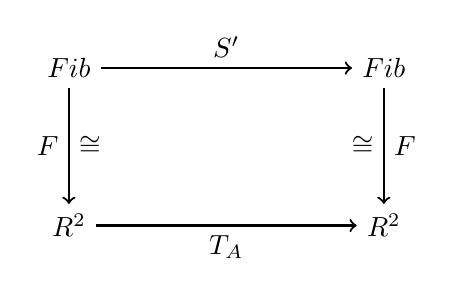
\begin{tikzpicture}[node distance=3cm, auto, thick]
    \node (Fib1) {$Fib$};
    \node (Fib2) [right of=Fib1, node distance=4cm] {$Fib$};
    \node (R1) [below of=Fib1, node distance=2cm] {$\mathbb{R}^2$};
    \node (R2) [below of=Fib2, node distance=2cm] {$\mathbb{R}^2$};

    \draw[->] (Fib1) to node {$S'$} (Fib2);
    \draw[->] (Fib1) to node[swap] {$F$} node {$\cong$} (R1);
    \draw[->] (Fib2) to node {$F$} node[swap] {$\cong$} (R2);
    \draw[->] (R1) to node[swap] {$T_A$} (R2);
  \end{tikzpicture}
\end{center}

\subsection{Eigenvalues and Eigenvectors}

The problem of finding a geometric sequence $(1, \lambda, \lambda^2, \dots)$ inside $Fib$ is equivalent to finding sequences that only scale by $\lambda$ when shifted. That is, we seek vectors $v$ such that $S'(v) = \lambda v$.

\begin{definition}[Eigenvalues and Eigenvectors]
  Let $V$ be a vector space and $T \in \End(V)$. A scalar $\lambda \in K$ is called an \qt{eigenvalue} of $T$ if there exists a non-zero vector $v \in V$ such that:
  \[ T(v) = \lambda v. \]
  The vector $v$ is called an \qt{eigenvector} associated with the eigenvalue $\lambda$.
\end{definition}

In the context of the Fibonacci matrix $A = \left(\begin{smallmatrix} 0 & 1 \\ 1 & 1 \end{smallmatrix}\right)$, calculating the roots of the characteristic polynomial reveals the eigenvalues to be the Golden Ratio $\varphi = \frac{1+\sqrt{5}}{2}$ and its conjugate $\psi = \frac{1-\sqrt{5}}{2}$. Their associated eigenvectors span $Fib$, leading directly to the closed-form Binet formula for the sequence. This forms the primary motivation for the upcoming deeper study of eigenvalues and determinants.